\chapter{BACKGROUND}

Our work concerns the investigation of complex computer vision problems using
the method of extracting deep hierarchical representations known as deep
learning.
In our articles we consider the relation of vision and natural language, and
apply deep learning to a challenging pixelwise tracking problem.
Underpinning the methods in our articles are a set of deep learning
architectures, each of which constitutes its own active topic of research.
After briefly describing deep learning as a whole, we introduce the particular
subcomponents underlying our models, in order to provide additional background
context before presenting our articles.


\section{Deep Learning}

Deep learning is a subfield of machine learning that uses a hierarchy of neural
network layers for representation learning~\cite{lecun2015deeplearning}.
Representation learning, then, means to extract from raw data meaningful
information in the form of vectors or tensors of real-valued numbers, called
``features''.
The defining quality of deep learning is its learning of a deep hierarchy of
representations using backpropagation~\cite{rumelhart1988learningreps}, which
is the term used by the deep learning community for reverse-mode automatic
differentation~\cite{griewank2008evaluatingderivatives}.
Thanks to breakthroughs in computation, data and algorithms, in recent years
deep learning methods have made progress in domains that had previously proven
challenging for traditional machine learning approaches.
Today, deep learning is a top-performing approach for solving complex
machine-learning problems including image and speech recognition, language
translation and natural language understanding topics such as question
answering~\cite{lecun2015deeplearning}.

We introduce feedforward neural networks (FNNs) as a simple yet concrete
example of a deep learning model.
FNNs can be expressed as a sequence of hidden layers
\begin{equation}
\vec{h}_i = f_i({\matr{W}_i}^\top \vec{h}_{i - 1} + \vec{b}_i),
\label{eqn:background:fnn}
\end{equation}
where $\vec{h}_i$ is a hidden unit, $\matr{W}_i$ is the weight matrix of
layer~$i$ of the neural network, $\vec{b}_i$ is a bias vector and $f_i$ is a
non-linearity or link function, such as the sigmoid
function~$f(x) = 1/(1 + e^{-x})$ or ReLU~$f(x) = \max(x, 0)$.
We may consider~$h_0$ as the input feature vector to the FNN, and~$h_L$ as the
output prediction for an FNN with~$L$ layers.
As with other deep models, the representation capacity of FNNs can be tuned by
increasing the depth of the network, i.e., the total number of layers of the
form in Equation~\ref{eqn:background:fnn}, or by increasing the width of each
of the layers~$i$, i.e., the dimension of the hidden
representation~$\vec{h}_i$.

In our articles we make use of more complex neural network architectures than
FNNs, which may include FNNs as a subcomponent.
In particular we focus on convolutional neural networks, recurrent neural
networks, attention networks, and fusion operators, all of which we describe
below.


\section{Convolutional Neural Networks}

Convolutional neural networks (CNNs) are a type of neural network designed to
model data that is arranged in a grid, as the pixels in an image are arranged.
While each neuron in a layer of an FNN is connected to all neurons in its
previous layer via a weight matrix, neurons in a layer of a CNN are only
locally connected to neurons in the previous layer.

We explain the meaning of ``locally connected''. We assume that a given layer
has a 3D tensor $\tens{V}$ as input, where in addition to the single dimension
of the hidden unit vector $\vec{h}$ of FNNs, there are two extra spatial
dimensions (e.g. $x$ and $y$ dimensions of an image).  A CNN connects the input
tensor $\tens{V}$ to an output tensor $\tens{Z}$ through a 4D tensor
$\tens{K}$ called a ``kernel'', which contains the CNN's learned parameters.

The kernel has one dimension matching the ``channels'' (the third, i.e.\
non-spatial, dimension of the input tensor $\tens{V}$), one dimension that
becomes the channels of the output tensor $\tens{Z}$, and two spatial
dimensions that are normally much smaller than the input feature tensor
$\tens{Z}$'s spatial dimensions. E.g.\ for an input image of dimensions $224
\times 224$ pixels and~\num{3} colour channels, a CNN kernel's spatial
dimensions would normally be $3 \times 3$. The CNN kernel's weights are thus
shared spatially, and each element of the output tensor is contributed to only
by a $3 \times 3$ spatial region of the input tensor, via a sum over dot
products on the vectorized slice of the kernel and the vectorized slice of the
spatial region.

Formally, each element $\tens{Z}_{i, j, k}$ of the output tensor corresponds to the
sum given in Equation~\ref{eqn:convolution}, where~$i$ is the index of the
output channel and $j$ and $k$ are the spatial indices of the output
element.\footnotemark{}
The index~$l$ runs over the input channels, while~$m$ and $n$ are restricted by
the spatial dimensions of the kernel, e.g.\ in our $3 \times 3$ kernel example
we have $m, n \in \{-1, 0, 1\}$.
\footnotetext[1]{Note that while CNNs are called ``convolutional'',
                 Equation~\ref{eqn:convolution} technically describes
                 cross-correlation.
                 True convolution in the sense of signal processing would be
                 identical to cross-correlation, except for a \ang{180}
                 rotation of the spatial slice of the kernel
                 weights~\cite{lyons1996understandingdsp}.
                 This technicality is inconsequential in machine learning,
                 since our weight initialization techniques generally do not vary under
                 rotation, and learned weights would adapt to accomodate the
                 rotation during training.}

\begin{equation}
        \tens{Z}_{i, j, k} = \sum_{l, m, n} \tens{V}_{l, j + m, k + n} \tens{K}_{i, l, m, n}
\label{eqn:convolution}
\end{equation}

\begin{figure}
\centering
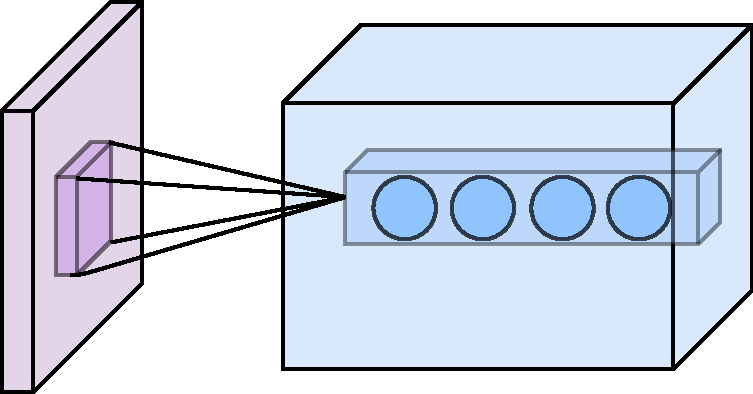
\includegraphics[width=1.0\textwidth]{Figures/cnn.pdf}
\caption{Two subsequent layers of a convolutional neural network.}
\label{fig:cnn}
\end{figure}

Figure~\ref{fig:cnn} depicts the interaction between two subsequent layers of a
CNN\@. The kernel~$\tens{K}$ (inner box on the left) is multiplied with a
volume of the input~$\tens{V}$ (outer box on the left) to produce a single unit
consisting of a column of values at a single spatial location in the
output~$\tens{Z}$.

CNNs generalize well in comparison to FNNs on visual data, since the number of
parameters are dramatically reduced compared with an equivalent FNN by sharing
parameters in the spatial dimensions~\cite{lecun-89}. This is an example of
improving generalization of neural networks by using prior knowledge (i.e.\ in
this case, the spatial equivariance of image data) when constructing a model
for a given type of data.

In the case of the visual question-answering task, we make use of a particular
CNN architecture called a ResNet~\cite{he2016deep} that has~\num{152} layers.
This CNN architecture has been pre-trained on a large dataset of image data to
extract useful generic feature representations from images.
The fusion operator takes this image feature representation as input, along
with a feature representation of the question, in order to predict an answer to
the posed question conditioned on the image.


\section{Recurrent Neural Networks}

Like CNNs, Recurrent Neural Networks~(RNNs)~\cite{rumelhart1986learning} are a
type of neural network model that has been designed using prior knowledge of
the type of data distribution relevant to the given task.
In particular, RNNs are designed to work on sequential data of arbitrary
length, such as time-series data including stock prices over time, or language
data, where the inputs are the word or character tokens making up sentences and
paragraphs.

Instead of sharing parameters spatially as in CNNs, RNNs share parameters over
time.
RNNs compute on variable-length sequence recursively, by computing a ``hidden
state''~$\vect{h}{t}$ activation at each timestep of an input sequence using
the input from the current timestep and the hidden state of the previous
timestep.
Formally,
\begin{equation}
\vect{h}{t} = \phi\big(\vect{h}{t - 1}, \vect{x}{t}\big),
\label{eqn:highlevel-rnn}
\end{equation}
where~$\phi$ represents the function defined by a particular recurrent unit.

In its basic form, the vanilla RNN,~$\phi$ may be as simple as the~$\tanh$ or
sigmoid nonlinearity of an affine combination of~$\vect{h}{t - 1}$
and~$\vect{x}{t}$.
In this vanilla RNN case, the pre-activation~$\vect{a}{t}$ at each timestep~$t$
is constructed from both the hidden state from the previous
timestep~$\vect{h}{t - 1}$ as well as the input~$\vect{x}{t}$ of the current
timestep, as given by Equation~\ref{eqn:vanilla-rnn},

\begin{equation}
        \vect{a}{t} = \matr{W}\vect{h}{t - 1} + \matr{U}\vect{x}{t} + \vec{b},
\label{eqn:vanilla-rnn}
\end{equation}
where~$\matr{W}$,~$\matr{U}$ and~$\vec{b}$ are the shared parameters of the
RNN\@.
The hidden state~$\vect{h}{t}$ is related to the pre-activation~$\vect{a}{t}$
of a given timestep~$t$ by the link function $f$,
i.e.\ $\vect{h}{t} = f(\vect{a}{t})$, where $f$ is usually~$\tanh$.


\section{Skip-Thought Vectors}

Skip-thought vectors~\cite{kiros2015skip} is a method of encoding a feature
representation from a sentence, in such a way that the feature representation
can be re-used as a generic, continuous sentence representation in a variety of
tasks.
In skip-thought vectors, an ``encoder'' RNN is trained to extract a feature
representation with enough context from the current sentence in order to
predict words in the sentences immediately preceding and following the current
sentence.

As their basic neural network component, skip-thought vectors use a type of RNN
called a Gated Recurrent Unit (GRU)~\cite{cho2014ontheproperties}.
Vanilla RNNs typically propagate information forward through time through an
alternating sequence of affine transformations and saturating nonlinearities.
In backpropagation through the resulting vanilla RNN computation graph,
gradients must sequentially traverse as many saturating nonlinearities as there
are timesteps, which causes the vanishing gradient problem.
Cho et al.\ designed GRUs to improve over the vanilla RNN activation
function in order to alleviate vanishing gradients in
RNNs~\cite{cho2014ontheproperties} using a similar mechanism to
skip-connections, which improve gradient flow in ResNets~\cite{he2016deep}.
Just as skip-connections compute each layer's activation as the weighted sum of
its input and a function of that input, GRUs do the same for each timestep's
activation.
GRUs allow gradients to backpropagate without traversing saturating
nonlinearities, by computing their hidden states~$\vect{h}{t}$ as the linear
interpolation between a candidate hidden state~$\vect{\widetilde{h}}{t}$ and
the previous hidden state~$\vect{h}{t - 1}$.

In order to compute the linear interpolation between previous and candidate
hidden states, GRUs include an update gate~$\vect{z}{t}$, defined as

\begin{equation}
\vect{z}{t} = \sigma\big(\matr{U}_z\vect{h}{t - 1} + \matr{W}_z\vect{x}{t}\big),
\label{eqn:gru-update-gate}
\end{equation}
where $\sigma(\cdot)$ is the sigmoid function.
The hidden state, then, is computed as
\begin{equation}
\vect{h}{t} = \big(1 - \vect{z}{t}\big) \odot \vect{h}{t - 1} + \vect{z}{t} \odot \vect{\widetilde{h}}{t}.
\label{eqn:gru-update}
\end{equation}

GRUs compute candidate hidden state~$\vect{\widetilde{h}}{t}$ similarly to
the vanilla RNN's hidden state given by Equation~\ref{eqn:vanilla-rnn},
except for the inclusion of a reset gate~$\vect{r}{t}$.
The reset gate varies between zero and one.
When the reset gate is near one, the candidate hidden state acts as the vanilla
RNN hidden state defined in Equation~\ref{eqn:vanilla-rnn}.
When the reset gate is near zero, the previous hidden state is ignored and the
candidate hidden state is computed solely from the current input.
Formally,

\begin{equation}
\vect{\widetilde{h}}{t} = f\big(\matr{W}\vect{h}{t - 1} + \vect{r}{t}\odot\big(\matr{U}\vect{x}{t}\big) + \vec{b}\big)
\end{equation}
where~$f$ is a nonlinearity, usually~$\tanh$.
Another set of parameters~$\matr{U}_r$ and~$\matr{W}_r$ compute~$\vect{r}{t}$
just as~$\matr{U}_z$ and~$\matr{W}_z$ compute~$\vect{z}{t}$ in
Equation~\ref{eqn:gru-update-gate}, i.e.,
$\vect{r}{t} = \sigma\big(\matr{U}_r\vect{h}{t - 1} + \matr{W}_r\vect{x}{t}\big)$.

Skip-thought vectors use an RNN, in our case a GRU, as an encoder, which
encodes the sequence of words in a sentence into a feature representation
corresponding to that sentence.
In our first article, we use skip-thought vectors to extract a feature
representation from the question, which is coupled with the feature
representation extracted from the image as a dual input to a multi-modal fusion
operator.
The multi-modal fusion operator takes the two feature-representation inputs and
produces an output prediction as to the answer to the given question,
conditioned on the image.
For the purposes of our first article, our multi-modal fusion operator predicts
a categorical variable, which represents a multiple-choice style answer.


\section{Attention}

Attention in deep learning is an operator motivated by the idea that making
predictions for a given task may require weighing a subset of inputs more
heavily than others, or even focusing on a single subset of inputs exclusive of
all others.
In vision, attention is motivated by the human fovea, which is responsible for
our sharp central vision used for demanding vision tasks such as driving and
reading.
In natural language, we structure our sentences differently depending on which
cues in our environment capture our focus~\cite{myachykov2005attention}.

The deep learning community drew inspiration from the importance of attention
in human perception, with early work using Boltzmann machines to combine foveal
glimpses~\cite{larochelle2010learning}, and using foveated images for
recognition and tracking~\cite{denil2012learning}.
Graves used differentiable attention in the form of weights of a mixture of
Gaussians over shifts for handwriting synthesis~\cite{graves2013generating}.
Mnih et al.\ used non-differentiable attention trained with reinforcement
learning to perform classification with reduced computation by observing only
predicted regions of an image~\cite{mnih2014recurrent}.
Bahdanau et al.\ introduced attention models for neural machine translation,
by predicting a set of weights~$(\alpha_1, \dots, \alpha_t)$ over the sequence
of hidden state vectors~$(h_1, \dots, h_t)$ over~$t$ timesteps output by an
encoder-decoder architecture~\cite{cho2014ontheproperties}.

In the following we describe mathematically the attention operator relevant to
this thesis.
We first introduce attention on sequences, i.e., 1D attention, before
describing our generalization to the spatiotemporal domain in our second
article.


\subsection{Scaled Dot-Product Attention}

Suppose we are given two matrices~$Q$ and~$K$ in~$\mathbb{R}^{t_1 \times c}$
and~$\mathbb{R}^{t_2\times c}$, respectively, defined
as~$Q \equiv (q_1, \dots, q_{t_1})$ and~$K \equiv (k_1, \dots, k_{t_2})$.
$Q$ and~$K$ represent input sequences of $c$-vectors, for example sequences of
word embeddings.
We wish to compute an output sequence~$Y \equiv (y_1, \dots, y_{t_1})$ that is
a linear combination of a third sequence~$V \equiv (v_1, \dots, v_{t_2})$ whose
weights in the linear combination depend on the affinity between pairs of
vectors in~$Q$ and~$K$.

In their work introducing Transformers for NLP tasks, Vaswani et
al.~\cite{vaswani2017attention} interpreted attention in the framework of data
retrieval, and we follow their perspective here.
An attention layer retrieves vector elements of the value~$V$ based on the
similarity of a query vector element from~$Q$ with the key vector from~$K$ that
corresponds to the value.
From our perspective, attention is a method for using query~$Q$ to perform a
lookup in the values~$V$, indexed by the key~$K$.

In particular, output vectors~$y_t \in \mathbb{R}^c$ are a linear combination
of all value vectors~$v_i$, with the weighting of~$v_i$ in the linear
combination dependent on the similarity of query vector~$q_t$ with key
vector~$k_i$.
At this point in our definition of attention we are faced with a decision about
how we should quantify the similarity between query vector~$q_t$ and key
vector~$k_i$.
Vaswani et al.\ refer to the similarity between query and key as attention's
``compatibility function''.
One possible compatibility function would be the ``additive alignment model''
used by Bahdanau et al.~\cite{bahdanau2015neuralmt}, which computes
compatibility by concatenating query and key and using this concatenated vector
as input to a feedforward neural network.
Another possibility is to use a dot-product compatibility function, which
computes the compatibility between query and key as their dot product.

The dot-product compatibility function has similar theoretical complexity to
additive compatibility, but has the advantage of being able to compute all
pairwise query-key compatibilities in a single matrix
multiplication~$QK^\top$.
Matrix multiplication is highly optimized on modern compute hardware, and
therefore dot-product attention runs faster than additive attention out of the
box.
For this reason, we use dot product attention in our work.

Our overall attention function is therefore

\begin{equation}
\mathtt{Attention}\big(Q, K, V\big) = \softmax{}\left(\frac{QK^\top}{\sqrt{c}}\right) V.
\label{eqn:background:attndefn}
\end{equation}

In Equation~\ref{eqn:background:attndefn} we scale by the square root of the
dimension of query and key vectors~$\sqrt{c}$ in the argument to the softmax.
The intuition behind this scaled dot product attention, as given by Vaswani et
al., is that if scalar elements of query and key vector were drawn from
independent zero-mean, unit-variance distributions, then the magnitude of the
query-key dot product grows like the square root of their dimension.
Therefore for query-key combinations whose dimensions are large, without
scaling it is likely that the softmax would saturate early in training, causing
vanishing gradients.


\subsection{Multi-Head Attention}

Building on scaled dot-product attention, multi-head attention is another
technique to improve the capacity while reducing the computation of attention.
Multi-head attention breaks the attention computation up into multiple
attention computations determined by the ``number of attention heads''
hyperparameter~$n_h$.
We illustrate multi-head attention in Figure~\ref{fig:background:multiheadattn}.

\begin{figure}
\centering
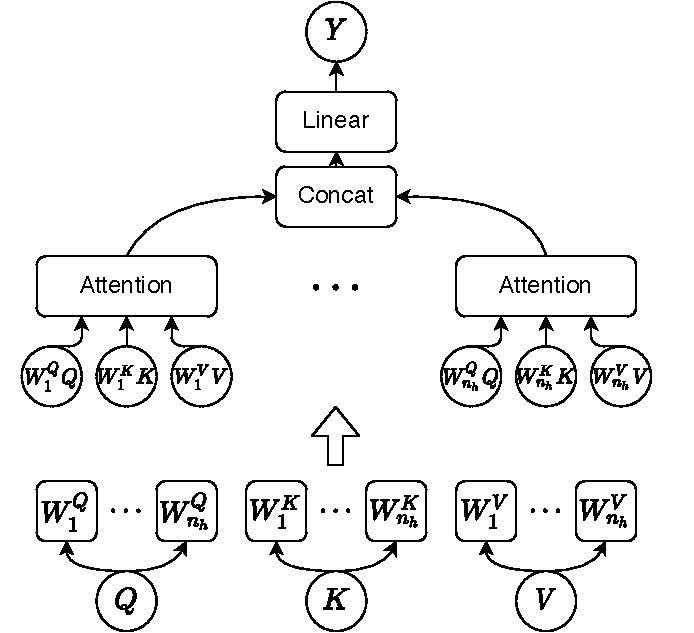
\includegraphics[width=0.8\textwidth]{Figures/multihead-attention.pdf}
\caption{Multi-head attention.
         Adapted from Vaswani et al.~\cite{vaswani2017attention}.}
\label{fig:background:multiheadattn}
\end{figure}

A single attention operator as given by Equation~\ref{eqn:background:attndefn}
would have a theoretical complexity proportional to the query and key
dimension~$c$.
In multi-head attention, we project query, key and value vectors by learned
weights~$W^Q_i \in \mathbb{R}^{c\times c/n_h}$,
$W^K_i \in \mathbb{R}^{c\times c/n_h}$,
and~$W^V_i \in \mathbb{R}^{c\times c/n_h}$, respectively, where~$i$
ranges from~$1$ to~$n_h$.
We then perform the~$n_h$ attention operations on the projected query, key and
value vectors.
Hence, multi-head attention on the projected vectors has the same theoretical
complexity as a single attention operator on the original query, key and value
vectors.
Intuitively, multi-head attention has the advantage that each~$i$th head can
specialize in learning to attend to particular features corresponding to the
affine subspace spanned by columns of the~$i$th projection weight matrix.

We concatenate outputs of the multi-head attention layers and feed the
resulting~$c$-vector into an output linear layer to produce the output~$Y$.
This final concatenation and projection step aggregates information from the
multiple attention heads, for example, to combine information gathered by
different attention heads ``looking at'' different regions of an image.


\subsection{Positional Encoding}

Up until this point in our description of attention, our attention operators
are unable to incorporate positional information, since query and key vectors
interact pairwise with each other.
While recurrent networks have a positional inductive bias, both convolutional
and attention networks are translation equivariant and require injection of
position information to perform position-dependent tasks such as
sequence-to-sequence learning.
Following Gehring et al.'s use of positional encodings for convolutional
sequence-to-sequence networks~\cite{gehring2017convolutional}, in Transformers
Vaswani et al.~\cite{vaswani2017attention} introduced positional encodings to
attention.

Positional encoding means adding to each key vector another vector with encoded
positional information.
Therefore with positional encoding Equation~\ref{eqn:background:attndefn} becomes

\begin{equation}
\mathtt{Attention}_E\big(Q, K, V\big) = \softmax{}\left(\frac{Q(K + E)^\top}{\sqrt{c}}\right) V,
\label{eqn:background:posenc-attn}
\end{equation}

\noindent where positional encoding matrix~$E \in \mathbb{R}^{t_2\times c}$ contains a
unique positional encoding~$c$-vector for each of the~$t_2$ elements in our
queried sequence.

We consider positional encodings constructed of learned embeddings, and sinusoidal
positional encodings.
In the case of learned embeddings, the positional encoding matrix~$E$ is
initialized at the beginning of training and updated along with the rest of the
model parameters using backpropagation.
Sinusoidal positional encodings, on the other hand, are not learned and instead
are fixed to a vector of values from a set of sinusoids of varying period
evaluated at the timestep, or sequence element,~$t$.
In particular,

\begin{equation}
\begin{split}
E_{t, 2i} &= \sin\left(\frac{t}{\tau^{2i/c}}\right) \\
E_{t, 2i + 1} &= \cos\left(\frac{t}{\tau^{2i/c}}\right)
\end{split}
\end{equation}

\noindent where~$\tau$ is a fixed constant, for example Vaswani et al.\ fixed~$\tau$
to~\num{10000}.

% TODO(brendan): attention in VQA and VOS

% \subsection{Sparse Attention}


% \subsection{Transformers}


\section{Fusion}

We refer to a topic specific to multimodal applications as fusion.
Following Lahat et al.'s definition~\cite{Lahat2015MultimodalDF}, multimodal
applications involve observing a single phenomenon using data collected from
multiple distinct sensors.
We refer to the raw stream of data collected from each sensor as a modality.
For example, we could treat a video as a multimodal application by making use
of RGB video frames, extracted optical flow and audio as input.
Autonomous driving also makes use of multimodal fusion to combine information
collected from multiple sensors, including LiDAR, radar, and camera
sensors~\cite{Feng2019DeepMO}.

Multimodal fusion refers to the technique by which information extracted from
these multiple raw data streams is combined.
Using fusion holds the promise of producing superior predictions by leveraging
the complementary information contained in separate data streams.
As an example proposed by Kazakos et al.~\cite{kazakos2019TBN}, consider an
egocentric action recognition system that is given as input a video of a person
at a kitchen sink.
When the sink tap is occluded, the audio signal provides a discriminative cue
for the actions ``turn tap on'' and ``turn tap off''.
On the other hand, video input would be more useful for predicting ``wiping
hands'', which has no discriminative auditory signal.
Hence, in this case multiple sensors provide the multimodal action recognition
system with complementary inputs leading to superior predictions.

Traditional multimodal fusion researcher categorize multimodal fusion
techniques into early and late fusion~\cite{ramachandram2017deepmultimodal}.
Early fusion involves combining modalities at the data level, which proves
challenging particularly for data drawn from sensors that may have different
sampling rates or resolutions.
Late fusion became popular in the early 2000s with the rise of ensemble
classifiers~\cite{kuncheva2004combining}.
Compared with early fusion, late fusion proves easier to implement, while
removing the need to retrain models pretrained on each modality, since late
fusion combines modalities at the prediction level.

Deep learning introduced a third category of multimodal fusion, ``intermediate
fusion'', made possible due to deep learning models' hierarchical
representations~\cite{ramachandram2017deepmultimodal}.
Since deep learning models have many layers, which collectively output a
hierarchical feature representation, deep models offer a flexible method for
performing fusion since representations from different modalities can be fused
at different levels of the representation hierarchy.
In deep multimodal models, separate modality-specific encoders, which could be
for example CNNs or RNNs, first extract representations from each modality
independently.
A ``fusion operator'' then combines the modality-specific representations into
a shared representation.

Fusion operators themselves have varying designs. A na\"ive approach would be to
concatenate the representations from different modalities and feed their
concatenation into a feedforward neural network to make a prediction.
However, this simple concatenation may lead to overfitting, and features
extracted from different modalities may be distributed differently so as to
make taking their affine combination an unfavourable fusion strategy.

In general, the subject of designing fusion operators that form effective
priors for combining modalities for a given task is a topic of active research.
Fusion operators are an important component, for example, in the visual
question answering (VQA)~\cite{fukui2016multimodalCB} and image hashtag
prediction~\cite{durand2020learninguserreps} domains.
Standard fusion operators include elementwise sum and product, and
concatenation.
Examples of research into more complex fusion operators include
MCB~\cite{fukui2016multimodalCB}, MUTAN~\cite{ben2017mutan},
GLU~\cite{dauphin2017languagemodeling} and TIRG~\cite{vo2019composing}.
Designing a search space over multimodal fusion operators for VQA is the topic
of our first article.
